\section{Analyse der Ist-Zustand der Barrierefreiheit der Desktopanwendungen}

\subsection{Barrierefreiheit in der Software-Entwicklung}
Blinde Menschen können keine Computermaus bedienen, d.h. dass die Software komplett per Tastatur bedienbar sein soll. Ein weiterer Grund, wieso Softwareunternehmen sich ebenfalls um digitale Barrierefreiheit kümmern sollten. Es ist eine harte Anforderung an Softwareentwickler, da es bezüglich des erwähnten Beispiels immer üblich war, die Software per Maus zu bedienen. Davon profitieren aber in dem Fall nicht nur Menschen mit Behinderungen. Funktioniert die Maus nicht mehr, so kann die Arbeit mit der Tastatur weitergehen. Programme, die eine Vorlesesoftware anbieten, können nur dann die graphische Oberfläche vorlesen, wenn sie mit Texten beschrieben wurde. Sogar Bilder sind davon betroffen. Ist die Oberfläche nicht gut beschriftet, so kann ein blinder Mensch oder auch Menschen mit Sehschwierigkeiten nichts erkennen. Für Menschen mit Seheinschränkungen ist beispielsweise ein Textcursor, der lediglich als senkrechter Strich im Eingabefeld dargestellt ist, nur schwer zu erkennen. Tastenkombinationen sind auch Barrieren, die für Menschen, die behinderungsbedingt nur eine Hand für das Bedienen der Software einsetzen können, die man durch die Individualisierbarkeit dieser Tastenkombinationen vermeiden kann. Individualisierbarkeit ist auch ein Begriff für Menschen mit Farbfehlsichtigkeit. Softwareunternehmen sollten die Möglichkeit anbieten, die Farben innerhalb der Software zu ändern. Da nicht jedes Unternehmen ihre Software auf digitale Barrierefreiheit testet, haben Menschen mit Behinderungen sehr geringe Auswahlmöglichkeiten.\footnote{PC Welt von IDG \cite{PcWelt}}

\subsection{Barrierefreiheit und Behindertengerecht}
\label{subsec:Barrierefreiheit und Behindertengerecht}
Häufig wird das Thema Barrierefreiheit so verstanden, dass es nur bestimmte Zielgruppen betrifft. Der Grund dafür ist, dass das Thema häufig mit Erkrankungen oder Unfällen verbunden wird, die einer offiziellen ärztlichen Diagnose bedürfen. In der Tat haben viel mehr Menschen ein Bedürfnis nach barrierefreier Software, als es ihnen selbst bewusst ist. In diesem Zusammenhang stellt sich unter anderem die Frage: Warum jeder digitale Barrierefreiheit braucht. Oftmals könnten Situationen jemanden einschränken, diese Situationen erfordern barrierefreien Zugang. Was einem nach dem letzten Satz sofort einfällt, sind Menschen mit Behinderungen, jedoch ist hier die Rede von jeder Einschränkung, selbst wenn sie nicht als Behinderung bezeichnet ist. Die \cref{fig:Beispielhafte Einschränkungen} zeigt diverse Einschränkungen, die nicht als Behinderungen zählen.\footnote{Katrin Borecki Usability Engineer, MACH AG \cite{mach}}

\begin{figure}[H]
	\centering
	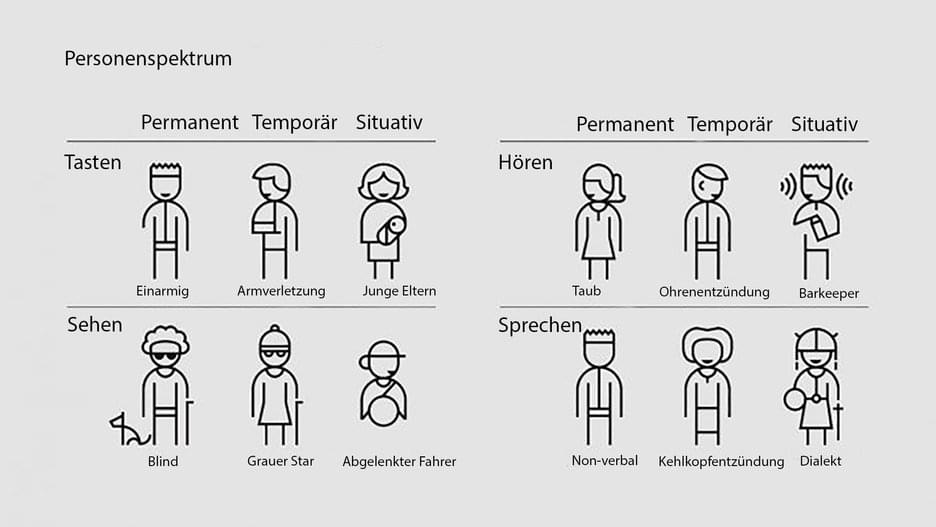
\includegraphics[width=1.0\textwidth]{Barrierefreiheit_personenspektrum}
	\caption[Personen mit verschiedenen Einschränkungen: Permanent, temporär und situativ]{Personen mit verschiedenen Einschränkungen: Permanent, temporär und situativ. 
	 Quelle: \cite{mach}}
	\label{fig:Beispielhafte Einschränkungen}
\end{figure}

Des Weiteren fühlen sich viele ältere Menschen nicht behindert. Sie stellen jedoch fest, dass die Schriften kleiner sind, der Kontrast geringer ist oder der Ton weniger laut ist als früher.\footnote{Ansatz zur Behebung von digitalen Barrieren \cite{giorgashvili2020nutzerzentrierter}}

\subsection{Prinzipien für digitale Barrierefreiheit}
\label{subsec:Prinzipien fuer Barrierefreiheit}

Sowohl die Normen der \ac{WCAG} 2.0 bzw. die \ac{WCAG} 2.1 als auch die \ac{BITV} 2.0 sind so aufgebaut, dass jeder Richtlinie dieser Normen eines der vier Prinzipien zugewiesen wird. Die vier Prinzipien stellen die Grundlagen der digitalen Barrierefreiheit dar und diese sind:

\begin{description}
	\item [Wahrnehmbar]\hfill \\
	Es geht darum, dass Informationen und Bestandteile einer \ac{GUI} den Benutzern so präsentiert werden, dass Benutzer sie wahrnehmen 
	können.\footnote{Web Content Accessibility Guidelines 2.0 \cite{WCAG2.0}}
	
	Ein Beispiel für die Wahrnehmung von Inhalten ist das Kontrastverhältnis zwischen dem Inhaltsfarbe und der Hintergrundsfarbe. Das betrifft alle 
	mögliche Elemente der \ac{GUI} außer Logos und beiläufigen Texten. Ein praktisches Beispiel zeigt die \cref{fig:Contrast ratio}:\footnote{Web Accessibility 
	Initiative \cite{WAI}}
	
	\begin{figure}[H]
		\centering
		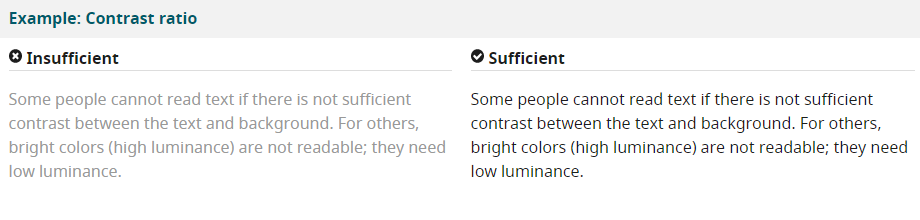
\includegraphics[width=1.0\textwidth]{Contrast ratio}
		\caption[Contrast ratio]{Contrast ratio \\Quelle: \cite{WAI}}
		\label{fig:Contrast ratio}
	\end{figure}
	
	Ein anderes Beispiel ist das ausschließliche Verwenden von Farben.. Bestimmte Zielgruppen können den angebotenen Inhalt gar nicht wahrnehmen. Die 
	\ref{fig:using color alone} veranschaulicht das erwähnte Beispiel:\footnote{Web Accessibility Initiative \cite{WAI}}
	
	\begin{figure}[H]
		\centering
		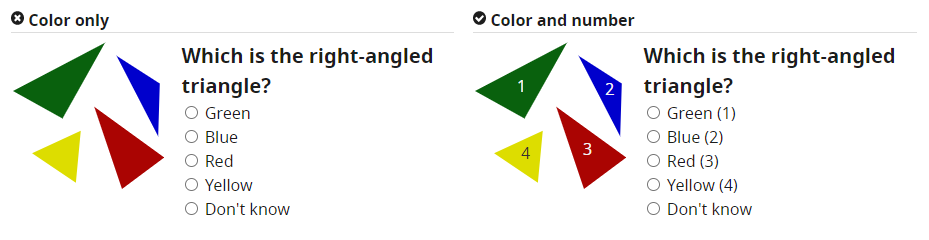
\includegraphics[width=1.0\textwidth]{Farben}
		\caption[Using color alone]{Using color alone \\Quelle: \cite{WAI}}
		\label{fig:using color alone}
	\end{figure}
	
	\item [Bedienbar]\hfill \\
	Alle Bestandteile der \ac{GUI} sowie die Navigation in dieser \ac{GUI} müssen bedienbar sein.\footnote{Web Content Accessibility Guidelines 2.0 \cite{WCAG2.0}}
	
	Beispiele für die Bestandteile der \ac{GUI} sind Links, Buttons und alle anderen interaktiven Inhalte, die z.B. den Fokus von mehreren Eingabemethoden erhalten 
	können. Diese können z.B. je nach Eingabemethode unterschiedliche Zustände bekommen, wie in \cref{fig:Ein Stile für verschiedene Linkszustände} dargestellt 
	ist:\footnote{Web Accessibility Initiative \cite{WAI}}
	
	\begin{figure}[H]
		\centering
		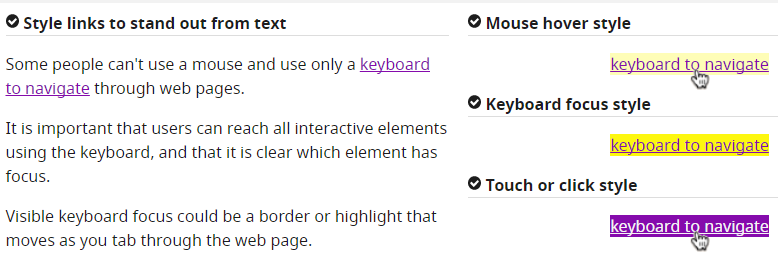
\includegraphics[width=1.0\textwidth]{Unique styles for different link states}
		\caption[Ein Stile für verschiedene Linkszustände]{Ein Stile für verschiedene Linkszustände \\Quelle: \cite{WAI}}
		\label{fig:Ein Stile für verschiedene Linkszustände}
	\end{figure}
	
	
	\item [Verständlich]\hfill \\
	Informationen und Bedienung der \ac{GUI} müssen den Benutzern in einer verständlichen Form präsentiert 
	werden.\footnote{Web Content Accessibility Guidelines 2.0 \cite{WCAG2.0}}
	
	Unverständliche Informationen bringen niemanden weiter. Wird beispielsweise etwas vom Nutzer verlangt oder dem Nutzer unterläuft ein Fehler, muss dem Nutzer ein entsprechendes 
	Feedback geliefert werden, so dass dieser nicht selbst nach dem Fehler suchen muss. Eine sehr bekannter Anwendungsfall, der einem regelmäßig begegnet, 
	ist die digitale Formularübermittlung. Bei einer fehlerhaften Benutzereingabe sucht der Benutzer lange nach dem Fehler, außer der Benutzer erhält entsprechendes 
	Feedback, dass den Fehler und den Standort des Fehlers beschreibt. Die \cref{fig:Using error list} zeigt das erwähnte Beispiel:\footnote{Web Accessibility Initiative \cite{WAI}}
	
	\begin{figure}[H]
		\centering
		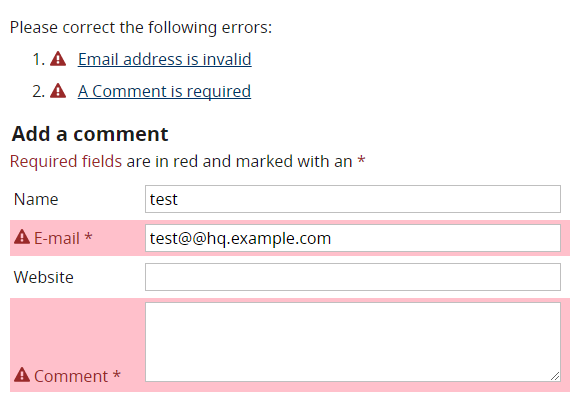
\includegraphics[width=1.0\textwidth]{Using error list}
		\caption[Verwendung von Fehlerliste, Symbol und Hintergrundfarbe, um Fehler zu markieren]{Verwendung von Fehlerliste, Symbol
		 und Hintergrundfarbe, um Fehler zu markieren. Quelle: \cite{WAI}}
		\label{fig:Using error list}
	\end{figure}
	
	\item [Robust]\hfill \\
	"`Inhalte müssen robust genug sein, damit sie zuverlässig von einer großen Auswahl an Benutzeragenten einschließlich assistierender Techniken 
	interpretiert werden können"'.\footnote{Web Content Accessibility Guidelines 2.0 \cite{WCAG2.0}}
	
	Um es überhaupt zu ermöglichen, dass z.B. assistierende Techniken funktionieren, müssen Komponenten der \ac{GUI} durch einen guten Namen, der beschreibt, was die Komponente
	ist/macht, versehen werden. Außerdem müssen Programmierer die richtigen Komponenten nehmen. Beispielsweise verhindert die Verwendung eines Bilds als Button die Verwendung 
	der assistierenden Techniken. Das folgende \textit{HTML-Code} verdeutlicht, was genau gemeint ist:
	
	Das Verwenden eines Bilds als Button:
	
	{\color{blue}
	\begin{verbatim}
		<img src="go.gif" onclick="goTo();" />
	\end{verbatim}}
	
	Stattdessen das Input-Element verwenden:
	
	{\color{blue}
	\begin{verbatim}
		<input type="button" value="go" name="Nächste_Seite_Button" />
	\end{verbatim}}
	
\end{description}

Unter den vier Prinzipien befinden sich die Richtlinien, die eine bestimmte Anzahl an testbaren Erfolgskriterien enthalten. Den Aufbau der erwähnten Normen veranschaulicht die \cref{fig:Aufbau der Normen}:\footnote{Das Konzept der \ac{WCAG} 2.0 und der \ac{BITV} 2.0 \cite{AufbauDerNormen}}

\begin{figure}[H]
	\centering
	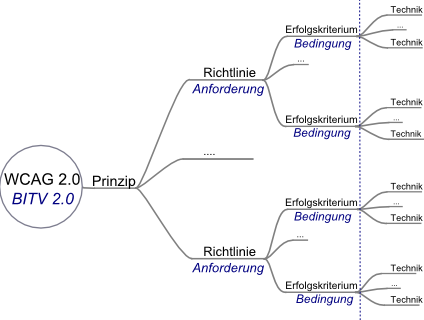
\includegraphics[width=0.8\textwidth]{Aufbau der Normen}
	\caption[Das Konzept der \ac{WCAG} 2.0 und der \ac{BITV} 2.0]{Das Konzept der \ac{WCAG} 2.0 und der \ac{BITV} 2.0 \\Quelle: \cite{AufbauDerNormen}}
	\label{fig:Aufbau der Normen}
\end{figure}

Wie in der \cref{fig:Aufbau der Normen} zu sehen ist, sind die Zweige ganz rechts Techniken. Diese sind zur Beseitigung der digitalen Barrieren von Erfolgskriterien.

\subsection{Konformitätsstufen anhand der \ac{WCAG}}
\label{subsubsec: Konformitätsstufen}
Nach den Richtlinien der \ac{WCAG} für Barrierefreiheit unterscheidet sich die Umsetzung der Anforderungen an barrierefreie Software in verschiedene Niveaus, die in drei Konformitätsstufen abgestuft sind. Diese sind:

\begin{description}
	\item [Konformitätsstufen A:] Die minimale Konformitätsstufe. Es ist ein Muss, da Menschen sonst die Inhalte nicht wahrnehmen und bedienen können. Wenn
	Erfolgskriterien der Konformitätsstufe A verletzt werden, dann ist mindestens eine Nutzergruppe von der Nutzung 
	ausgeschlossen.\footnote{Hochschule für Technik und Wirtschaft Dresden \cite{HV}}
	
	\item [Konformitätsstufen AA:] Sie ist in Europa und in Deutschland für öffentliche Stellen vorgegeben. Für eine Konformität auf dieser Stufe 
	müssen all Erfolgskriterien der Stufe \textbf{A} und der Stufe \textbf{AA} erfüllt werden. Sind die Erfolgskriterien dieser Stufe nicht umsetzbar, so
	müssen Alternativen dieser Erfolgskriterien
	zur Verfügung gestellt werden. Diese Stufe kann als angestrebte Norm bezeichnet werden, da Menschen sonst die Inhalte nur schwer wahrnehmen und bedienen 
	können.\footnote{Hochschule für Technik und Wirtschaft Dresden \cite{HV}}
	
	\item [Konformitätsstufen AAA:] Um auf diese Stufe zu kommen, müssen zuerst die ersten zwei Stufen \textbf{A} und \textbf{AA} erfüllt werden. "`Kein 
	Webauftritt wird jemals realistischerweise alle WCAG Erfolgskriterien auch der Konformitätsstufe AAA erfüllen. Nicht einmal die WAI empfiehlt, sich 
	dieses Ziel vorzunehmen. Es wird nicht empfohlen, Konformität auf Stufe AAA als allgemeine Richtlinie für komplette Websites zu fordern, da es bei manchen
	Inhalten nicht möglich ist, alle Erfolgskriterien der Stufe AAA zu erfüllen."'\footnote{Zweiter Blick \cite{ZweiterBlick}}
\end{description}

Zur besseren Vorstellung dieser Konformitätsstufen kann \cref{fig:Konformitätsstufen} \footnote{Hochschule für Technik und Wirtschaft Dresden \cite{HV}} beitragen.

\begin{figure}[H]
	\centering
	\includegraphics[width=1.0\textwidth]{Konformitätsstufen}
	\caption[Konformitätsstufen nach der \ac{BITV} 2.0]{Konformitätsstufen nach der \ac{BITV} 2.0 \\Quelle: \cite{HV}}
	\label{fig:Konformitätsstufen}
\end{figure}

\vspace{2cm}

Es bestehen jedoch Ausnahmen für Technologien, die nicht barrierefrei sind und trotzdem unter den folgenden Bedingungen eingesetzt werden dürfen:\footnote{Web Content Accessibility Guidelines 2.1 \cite{WCAG2.1}}

\begin{itemize}
	\item Falls die Inhalte parallel in einer barrierefreien Version zur Verfügung gestellt werden können.
	\item Solange die Anforderungen der Barrierefreiheit erfüllt sind, können andere Elemente die Wahrnehmung, Bedienbarkeit oder das Verständnis nicht 
	stören. Solche Elemente sind Nicht-Störende-Elemente genannt.
\end{itemize}

\subsection{Normen der \ac{WCAG} 2.0}
Die \ac{WCAG} 2.0 sind der internationale Webstandard des \ac{W3C}s zur barrierefreien Gestaltung von Internetseiten. Ab 23. September 2019 gelten die \ac{WCAG} 2.0 in der Europäischen Union für neue Webseiten und ab 23. September 2020 für bestehende Webseiten. In Deutschland wird seit 2002 die Umsetzung der \ac{WCAG} 2.0 durch die gesetzliche Verankerung in der \ac{BITV} gefördert. Die \ac{WCAG} 2.0 legen Erfolgskriterien fest, um die Konformität zu definieren.\footnote{Web Content Accessibility Guidelines 2.0 \cite{WCAG2.0}}

Es werden alle Richtlinien und ihre Erfolgskriterien der \ac{WCAG} 2.0 betrachtet, allerdings werden in \cref{subsec: Umsetzbare Kriterien} die Kriterien ausgewählt, die einen Einfluss 
auf die Desktopanwendungen haben und die in der aktuellen Software der AKG Software Consulting GmbH umsetzbar sind.

Jede Richtlinie gehört einem der vier Prinzipien der digitalen Barrierefreiheit an, was in der Aufzählung der Richtlinien im Folgenden zu sehen ist. Außerdem wird jedem Erfolgskriterium  eine Konformitätsstufe zugewiesen.

\begin{description}
	\item[Richtlinie 1.1 Textalternativen]\hfill
	\begin{itemize}
		\item \textbf{Prinzip:} Wahrnehmbar.
		\item \textbf{Allgemeine Beschreibung:} Für alle Nicht-Text-Inhalte müssen Textalternativen zur Verfügung gestellt werden, damit der Benutzer die
		präsentierte Form der Inhalte nach seinem Bedürfnis ändern kann.\footnote{Web Content Accessibility Guidelines 2.0 \cite{WCAG2.0}}
	\end{itemize}
	
	\begin{description}
		\item[Erfolgskriterium 1.1.1 Nicht-Text-Inhalt]\hfill
		\begin{itemize}
			\item \textbf{Konformitätsstufe:} A
			\item \textbf{Beschreibung:} Es müssen Mittel zum Ersetzen der Nicht-Text-Inhalte dargestellt werden können, so dass die
			Nicht-Text-Inhalte den Benutzer nicht behindern. Beispielsweise die Anpassung der Schriftgröße, die Verwendung von Symbolen oder Brailleschrift sowie die Umwandlung der Texte 
			in eine einfachere Sprache. Das sind alles Mittel, die zu Textalternativen zählen.
			Nichtsdestotrotz gibt es dafür Ausnahmen: Steuerelemente oder Eingaben durch den Benutzer, da diese einen Namen haben, der den Zweck des Element
			beschreibt. Außerdem sind Tests und Übungen von diesem Erfolgskriterium ausgenommen, da ein alternativer Text eine deskriptive Identifizierung
			des Tests oder der Übung bereitstellt und so damit der Sinn des Tests bzw. der Übung entfällt. Wenn es sich um die Vermittlung/Schaffung bestimmter
			Sinneserfahrungen handelt, kann ein Nicht-Text-Element ohne Textalternativen präsentiert werden. Darüber hinaus sind \ac{CAPTCHA} von der Regel ausgenommen,
			denn es geht darum, vom Benutzer eine Bestätigung zu verlangen, dass überhaupt eine Person und kein Computer auf den Inhalt zugreift. Allerdings gibt
			es statt der Textalternativen für das Ersetzen von \ac{CAPTCHA}s andere Ausgabeformen, die der sensorischen Wahrnehmung nutzen. Unsichtbare Elemente
			oder reine Dekoration, die ausschließlich für visuelle Formatierung verwendet wird, müssen keine Textalternativen haben, dennoch müssen
			sie so implementiert werden, dass sie von assistierender Technik ignoriert werden können.\footnote{Web Content Accessibility Guidelines 2.0 \cite{WCAG2.0}}
		\end{itemize}
	\end{description}
	
	\item[Richtlinie 1.2 Zeitbasierte Medien]\hfill
	\begin{itemize}
		\item \textbf{Prinzip:} Wahrnehmbar.
		\item \textbf{Allgemeine Beschreibung:} Es geht darum, dass Alternativen zu den zeitbasierten Medien zur Verfügung gestellt werden müssen. Davon ausgenommen sind 
		Medien, die Alternativen zum Text sind.\footnote{Web Content Accessibility Guidelines 2.0 \cite{WCAG2.0}}
	\end{itemize}
	
	\begin{description}
		\item[Erfolgskriterium 1.2.1 Reine Audio- und Videoinhalte (aufgezeichnet)]\hfill
		\begin{itemize}
			\item \textbf{Konformitätsstufe:} A
			\item \textbf{Beschreibung:} Eine Alternative für reine aufgezeichnete Audio- und Videoinhalte, die äquivalente Informationen 
			liefert, muss bereitgestellt werden.\footnote{Web Content Accessibility Guidelines 2.0 \cite{WCAG2.0}}
		\end{itemize}
			
		\item[Erfolgskriterium 1.2.2 Untertitel (aufgezeichnet)]\hfill
		\begin{itemize}
			\item \textbf{Konformitätsstufe:} A
			\item \textbf{Beschreibung:} Für alle aufgezeichneten Audioinhalte in synchronisierten Medien müssen Untertitel bereitgestellt 
			werden.\footnote{Web Content Accessibility Guidelines 2.0 \cite{WCAG2.0}}
		\end{itemize}
			
		\item[Erfolgskriterium 1.2.3 Audiodeskription (aufgezeichnet)]\hfill
		\begin{itemize}
			\item \textbf{Konformitätsstufe:} A
			\item \textbf{Beschreibung:} Es müssen für synchronisierte Medien eine Audiodeskription des aufgezeichneten Videoinhalts oder andere 
			Medienalternativen zur Verfügung gestellt werden.\footnote{Web Content Accessibility Guidelines 2.0 \cite{WCAG2.0}}
		\end{itemize}
			
		\item[Erfolgskriterium 1.2.4 Untertitel (Live)]\hfill
		\begin{itemize}
			\item \textbf{Konformitätsstufe:} AA
			\item \textbf{Beschreibung:} Für alle Live-Audioinhalte müssen Untertitel bereitgestellt werden.\footnote{Web Content Accessibility Guidelines 2.0 \cite{WCAG2.0}}
		\end{itemize}
			
		\item[Erfolgskriterium 1.2.5 Audiodeskription (aufgezeichnet)]\hfill
		\begin{itemize}
			\item \textbf{Konformitätsstufe:} AA
			\item \textbf{Beschreibung:} Alle aufgezeichneten Videoinhalte in synchronisierten Medien müssen eine Audiodeskription 
			haben.\footnote{Web Content Accessibility Guidelines 2.0 \cite{WCAG2.0}}
		\end{itemize}
			
		\item[Erfolgskriterium 1.2.6 Gebärdensprache (aufgezeichnet)]\hfill
		\begin{itemize}
			\item \textbf{Konformitätsstufe:} AAA
			\item \textbf{Beschreibung:} Für alle aufgezeichneten Videoinhalte in synchronisierten Medien muss eine Übersetzung in die Gebärdensprache zur 
			Verfügung gestellt werden.\footnote{Web Content Accessibility Guidelines 2.0 \cite{WCAG2.0}}
		\end{itemize}
			
		\item[Erfolgskriterium 1.2.7 Erweiterte Audiodeskription (aufgezeichnet)]\hfill
		\begin{itemize}
			\item \textbf{Konformitätsstufe:} AAA
			\item \textbf{Beschreibung:} Sind die Pausen im Haupt-Audio für eine Audiodeskription nicht ausreichend, um den Sinn des Inhaltes zu vermitteln oder 
			wichtige Details zu beschreiben, dann ist für alle aufgezeichnete Videoinhalte in synchronisierten Medien eine erweiterte 
			Audiodeskription bereitzustellen.\footnote{Web Content Accessibility Guidelines 2.0 \cite{WCAG2.0}}
		\end{itemize}
			
		\item[Erfolgskriterium 1.2.8 Medienalternative (aufgezeichnet)]\hfill
		\begin{itemize}
			\item \textbf{Konformitätsstufe:} AAA
			\item \textbf{Beschreibung:} Für alle aufgezeichneten synchronisierten Medien muss eine Alternative für zeitbasierte Medien bereitgestellt 
			werden.\footnote{Web Content Accessibility Guidelines 2.0 \cite{WCAG2.0}}
		\end{itemize}
			
		\item[Erfolgskriterium 1.2.9 Reiner Audioinhalt (live)]\hfill
		\begin{itemize}
			\item \textbf{Konformitätsstufe:} AAA
			\item \textbf{Beschreibung:} Eine Alternative für zeitbasierte Medien muss zur Verfügung gestellt werden, die äquivalente Informationen 
			für live übertragene reine Audioinhalte anbietet.\footnote{Web Content Accessibility Guidelines 2.0 \cite{WCAG2.0}}
		\end{itemize}
			
	\end{description}

	\item[Richtlinie 1.3 Anpassbar]\hfill
	\begin{itemize}
		\item \textbf{Prinzip:} Wahrnehmbar.
		\item \textbf{Allgemeine Beschreibung:} Das Präsentieren der Inhalte muss auf verschiedene Arten ohne Verlust von Informationen oder 
		Struktur dargestellt werden können.\footnote{Web Content Accessibility Guidelines 2.0 \cite{WCAG2.0}}
	\end{itemize}
	
	\begin{description}
		\item[Erfolgskriterium 1.3.1 Informationen und Beziehungen]\hfill
		\begin{itemize}
			\item \textbf{Konformitätsstufe:} A
			\item \textbf{Beschreibung:} Falls Informationen, Struktur und Beziehungen über die Darstellung vermittelt werden, müssen diese durch Software bestimmt 
			oder in Textform bereitgestellt werden können.\footnote{Web Content Accessibility Guidelines 2.0 \cite{WCAG2.0}}
		\end{itemize}
			
		\item[Erfolgskriterium 1.3.2 Bedeutungstragende Reihenfolge]\hfill
		\begin{itemize}
			\item \textbf{Konformitätsstufe:} A
			\item \textbf{Beschreibung:} Wirkt sich die Reihenfolge der Inhalte auf die Bedeutung der Inhalte aus, so muss die korrekte Leseabfolge durch Software 
			bestimmt werden können. Mit einer korrekten Leseabfolge ist gemeint, dass die Reihenfolge der Inhalte deren Bedeutung nicht 
			verändert.\footnote{Web Content Accessibility Guidelines 2.0 \cite{WCAG2.0}}
		\end{itemize}
			
		\item[Erfolgskriterium 1.3.3 Sensorische Eigenschaften]\hfill
		\begin{itemize}
			\item \textbf{Konformitätsstufe:} A
			\item \textbf{Beschreibung:} Falls es Anweisungen gibt, die für das Verständnis und die Bedienung der Inhalte zur Verfügung stehen, müssen diese 
			nicht nur von sensorischen Eigenschaften der Komponenten abhängig sein, wie z.B. die visuelle Position oder die Größe des 
			Elements.\footnote{Web Content Accessibility Guidelines 2.0 \cite{WCAG2.0}}
		\end{itemize}
	\end{description}

	\item[Richtlinie 1.4 Unterscheidbar]\hfill
	\begin{itemize}
		\item \textbf{Prinzip:} Wahrnehmbar.
		\item \textbf{Allgemeine Beschreibung:} Den Benutzern muss es leichter fallen, Inhalt zu sehen und zu hören.\footnote{Web Content Accessibility Guidelines 2.0 \cite{WCAG2.0}}
	\end{itemize}
	
	\begin{description}
		\item[Erfolgskriterium 1.4.1 Benutzung von Farbe]\hfill
		\begin{itemize}
			\item \textbf{Konformitätsstufe:} A
			\item \textbf{Beschreibung:} Um Inhalte zu unterscheiden oder Informationen zu vermitteln, dürfen die Farben nicht als einziges Mittel benutzt 
			werden.\footnote{Web Content Accessibility Guidelines 2.0 \cite{WCAG2.0}}
		\end{itemize}
		
		\item[Erfolgskriterium 1.4.2 Audio-Steuerelement]\hfill
		\begin{itemize}
			\item \textbf{Konformitätsstufe:} A
			\item \textbf{Beschreibung:} Wird ein Audioinhalt auf der Webseite für mehr als 3 Sekunden abgespielt, dann wird die Möglichkeit angeboten, dass der 
			Benutzer dieses Element steuert. Entweder kann der Benutzer das Audioelement pausieren oder die Lautstärke des Audioelements unabhängig von der 
			allgemeinen Systemlautstärke regeln.\footnote{Web Content Accessibility Guidelines 2.0 \cite{WCAG2.0}}
		\end{itemize}
		
		\item[Erfolgskriterium 1.4.3 Kontrast (Minimum)]\hfill
		\begin{itemize}
			\item \textbf{Konformitätsstufe:} AA
			\item \textbf{Beschreibung:} Das Kontrastverhältnis von Text und Bilder, die Text enthalten, muss mindestens 4,5 zu 1 (4,5:1) sein. Falls der Text größer 
			als 14pt ist, dann muss das Kontrastverhältnis davon mind. 3 zu 1 (3:1) sein. Ausgenommen sind die rein dekorativen Inhalte (wenn sie keine Informationen
			 liefern).\footnote{Web Content Accessibility Guidelines 2.0 \cite{WCAG2.0}}
		\end{itemize}
		
		\item[Erfolgskriterium 1.4.4 Textgröße ändern]\hfill
		\begin{itemize}
			\item \textbf{Konformitätsstufe:} AA
			\item \textbf{Beschreibung:} Die Textgröße muss bis zu 200 Prozent ohne Verlust von Inhalt geändert werden können. Davon ausgenommen sind die 
			Untertitel und Bilder eines Textes.\footnote{Web Content Accessibility Guidelines 2.0 \cite{WCAG2.0}}
		\end{itemize}
		
		\item[Erfolgskriterium 1.4.5 Bilder eines Textes]\hfill
		\begin{itemize}
			\item \textbf{Konformitätsstufe:} AA
			\item \textbf{Beschreibung:} Falls mit der Darstellung von Bildern eines Textes Informationen verloren gehen können, wird Text statt Bilder eines Textes 
			benutzt.\footnote{Web Content Accessibility Guidelines 2.0 \cite{WCAG2.0}}
		\end{itemize}
		
		\item[Erfolgskriterium 1.4.6 Kontrast (erhöht)]\hfill
		\begin{itemize}
			\item \textbf{Konformitätsstufe:} AAA
			\item \textbf{Beschreibung:} Das Kontrastverhältnis von Text und Bilder eines Textes muss mindestens 7 zu 1 sein. Für größere Texte (größer als 14pt) bzw. 
			Bilder eines Textes ist das Kontrastverhältnis mindestens 4,5 zu 1. Analog zum Erfolgskriterium 1.4.3 sind die reinen dekorativen Inhalte von 
			der Regel ausgenommen.\footnote{Web Content Accessibility Guidelines 2.0 \cite{WCAG2.0}}
		\end{itemize}
		
		\item[Erfolgskriterium 1.4.7 Leiser oder kein Hintergrund-Audioinhalt]\hfill
		\begin{itemize}
			\item \textbf{Konformitätsstufe:} AAA
			\item \textbf{Beschreibung:} Aufgezeichneter Audioinhalt, der Sprache im Vordergrund hat, kein Audio-CAPTCHA oder Audio-Logo und auch kein musikalischer Ausdruck
			wie z.B. Singen ist, muss entweder abgeschaltet werden können oder gar keine Hintergrundgeräusche enthalten, oder die Hintergrundgeräusche sind mindestens 20 Dezibel 
			leiser als der Sprachinhalt im Vordergrund.\footnote{Web Content Accessibility Guidelines 2.0 \cite{WCAG2.0}}
		\end{itemize}
		
		\item[Erfolgskriterium 1.4.8 Visuelle Präsentation]\hfill
		\begin{itemize}
			\item \textbf{Konformitätsstufe:} AAA
			\item \textbf{Beschreibung:} Für die Darstellung von Textblöcken gilt:\footnote{Web Content Accessibility Guidelines 2.0 \cite{WCAG2.0}}
			\begin{itemize}
				\item Vorder- und Hintergrundfarben können geändert werden.
				\item Text ist nicht im Blocksatz ausgerichtet.
				\item Die Breite beträgt nicht mehr als 80 Zeichen.
				\item Innerhalb von Paragraphen ist der Zeilenabstand mindestens 1,5-fach und zwischen Paragraphen mindestens 1,5-fach so 
				groß wie der Zeilenabstand.
				\item Die Textgröße kann ohne zusätzliche Technik bis auf 200\% skaliert werden und das ohne, dass der Leser dafür scrollen muss.
			\end{itemize}
		\end{itemize}
		
		\item[Erfolgskriterium 1.4.9 Bilder eines Textes (keine Ausnahme)]\hfill
		\begin{itemize}
			\item \textbf{Konformitätsstufe:} AAA
			\item \textbf{Beschreibung:} Bilder eines Textes können nur dann benutzt werden, wenn sie entweder rein dekorativ sind oder wenn die Vermittlung von bestimmten 
			 Informationen anders nicht möglich ist. Ein Beispiel dafür ist der Text in einem Logo.\footnote{Web Content Accessibility Guidelines 2.0 \cite{WCAG2.0}}
		\end{itemize}
	\end{description}
	
	\item[Richtlinie 2.1 Per Tastatur zugänglich]\hfill
	\begin{itemize}
		\item \textbf{Prinzip:} Bedienbar.
		\item \textbf{Allgemeine Beschreibung:} Alle Funktionalitäten müssen per Tastatur erreichbar sein.\footnote{Web Content Accessibility Guidelines 2.0 \cite{WCAG2.0}}
	\end{itemize}
	
	\begin{description}
		\item[Erfolgskriterium 2.1.1 Tastatur]\hfill
		\begin{itemize}
			\item \textbf{Konformitätsstufe:} A
			\item \textbf{Beschreibung:} Durch eine Tastaturschnittstelle müssen alle möglichen Funktionalitäten bedienbar sein, ohne dass eine bestimmte 
			Zeiteinteilung für einzelne Tastenanschläge erforderlich ist. Eingabetechniken sind in diesem Zusammenhang nicht 
			gemeint.\footnote{Web Content Accessibility Guidelines 2.0 \cite{WCAG2.0}}
		\end{itemize}
		
		\item[Erfolgskriterium 2.1.2 Keine Tastaturfalle]\hfill
		\begin{itemize}
			\item \textbf{Konformitätsstufe:} A
			\item \textbf{Beschreibung:} Anhand der Tastaturschnittstelle muss der Tastaturfokus von einem Bestandteil zum anderen bewegt werden können. Außerdem wird, wenn 
			die üblichen Bewegungsmethoden von einem Bestandteil zum anderen abweicht, der Benutzer darüber informiert.\footnote{Web Content Accessibility Guidelines 2.0 \cite{WCAG2.0}}
		\end{itemize}
		
		\item[Erfolgskriterium 2.1.3 Tastatur (keine Ausnahme)]\hfill
		\begin{itemize}
			\item \textbf{Konformitätsstufe:} AAA
			\item \textbf{Beschreibung:} Analog zum Erfolgskriterium 2.1.1 nur ohne Ausnahmen.\footnote{Web Content Accessibility Guidelines 2.0 \cite{WCAG2.0}}
		\end{itemize}
	\end{description}
	
	\item[Richtlinie 2.2 Ausreichend Zeit]\hfill
	\begin{itemize}
		\item \textbf{Prinzip:} Bedienbar.
		\item \textbf{Allgemeine Beschreibung:} Der Benutzer erhält genügend Zeit, um Inhalte zu lesen und zu benutzen.\footnote{Web Content Accessibility Guidelines 2.0 \cite{WCAG2.0}}
	\end{itemize}
	
	\begin{description}
		\item[Erfolgskriterium 2.2.1 Zeiteinteilung anpassbar]\hfill
		\begin{itemize}
			\item \textbf{Konformitätsstufe:} A
			\item \textbf{Beschreibung:} Falls es zeitlich begrenzte Inhalte gibt, dann gilt für diesen Inhalt:
			\begin{itemize}
				\item Abschalten und Anpassen und das bevor der Benutzer auf diesen Inhalt trifft.
				\item Ausweiten der zeitlichen Begrenzung, bevor sie abläuft und zwar so, dass der Benutzer mind. 20 Sekunden vor Ablauf gewarnt wird. Der Benutzer muss 
				dementsprechend informiert werden, wie er die zeitliche Begrenzung ausweitet.
			\end{itemize}
			Es gelten für diese Richtlinie folgende Ausnahmen: Wenn es sich beispielsweise um Echtzeit-Inhalt handelt wie bei einer Auktion oder wenn die Ausweitung 
			der zeitlichen Begrenzung den Inhalt ungültig macht. Wenn die zeitliche Begrenzung mehr als 20 Stunden dauert, dann gilt diese nicht 
			mehr.\footnote{Web Content Accessibility Guidelines 2.0 \cite{WCAG2.0}}
		\end{itemize}
		
		\item[Erfolgskriterium 2.2.2 Pausieren, beenden, ausblenden]\hfill
		\begin{itemize}
			\item \textbf{Konformitätsstufe:} A
			\item \textbf{Beschreibung:} Für Inhalte, die sich automatisch bewegen, aktualisieren, scrollen und blinken (Wechseln zwischen mehreren Zuständen um den 
			Benutzer aufmerksam zu machen), muss der Benutzer sie steuern können, indem er sie pausieren, beenden und ausblenden kann, es sei denn, dass eine der 
			erwähnten Aktionen ein Teil einer Handlung ist, ohne die Informationen verloren gehen können.\footnote{Web Content Accessibility Guidelines 2.0 \cite{WCAG2.0}}
		\end{itemize}
		
		\item[Erfolgskriterium 2.2.3 Keine Zeiteinteilung]\hfill
		\begin{itemize}
			\item \textbf{Konformitätsstufe:} AAA
			\item \textbf{Beschreibung:} Es treten Keine zeitlich begrenzten Inhalte auf, es sei denn, dass es sich um Echtzeit Ereignisse (eine Auktion) oder  
			synchronisierte Medien handelt.\footnote{Web Content Accessibility Guidelines 2.0 \cite{WCAG2.0}}
		\end{itemize}
		
		\item[Erfolgskriterium 2.2.4 Unterbrechungen]\hfill
		\begin{itemize}
			\item \textbf{Konformitätsstufe:} AAA
			\item \textbf{Beschreibung:} Der Benutzer kann jede Unterbrechung aufschieben oder unterdrücken, es sei denn, dass es sich um einen Notfall 
			handelt.\footnote{Web Content Accessibility Guidelines 2.0 \cite{WCAG2.0}}
		\end{itemize}
		
		\item[Erfolgskriterium 2.2.5 Erneute Authentifizierung]\hfill
		\begin{itemize}
			\item \textbf{Konformitätsstufe:} AAA
			\item \textbf{Beschreibung:} Es geht darum, dass der Benutzer ohne Datenverlust nach der erneuten Authentifizierung (wenn die Sitzung abläuft) 
			fortfahren kann.\footnote{Web Content Accessibility Guidelines 2.0 \cite{WCAG2.0}}
		\end{itemize}
	\end{description}
	
	\item [Richtlinie 2.3 Anfälle]\hfill
	\begin{itemize}
		\item \textbf{Prinzip:} Bedienbar.
		\item \textbf{Allgemeine Beschreibung:} Die Gestaltung der Inhalte darf nicht zu Anfällen führen.\footnote{Web Content Accessibility Guidelines 2.0 \cite{WCAG2.0}}
	\end{itemize}
	
	\begin{description}
		\item[Erfolgskriterium 2.3.1 Grenzwert von dreimaligem Blitzen oder weniger]\hfill
		\begin{itemize}
			\item \textbf{Konformitätsstufe:} A
			\item \textbf{Beschreibung:} Webseiten dürfen keine Elemente/Inhalte haben, die mehr als dreimal in einem beliebigen, eine Sekunde dauernden Zeitraum 
			blitzen. Es gilt für diese Richtlinie eine Ausnahme und zwar wenn der Blitz unterhalb der allgemeinen Grenzwerte zu Blitzen und roten Blitzen liegt
			(siehe \nameref{subsec: Anlage1}).\footnote{Web Content Accessibility Guidelines 2.0 \cite{WCAG2.0}}
		\end{itemize}
		
		\item[Erfolgskriterium 2.3.2 Drei Blitze]\hfill
		\begin{itemize}
			\item \textbf{Konformitätsstufe:} AAA
			\item \textbf{Beschreibung:} Analog zum Erfolgskriterium 2.3.1 nur ohne Ausnahmen.\footnote{Web Content Accessibility Guidelines 2.0 \cite{WCAG2.0}}
		\end{itemize}
	\end{description}
	
	\item[Richtlinie 2.4 Navigierbar]\hfill
	\begin{itemize}
		\item \textbf{Prinzip:} Bedienbar.
		\item \textbf{Allgemeine Beschreibung:} Es werden dem Benutzer Mittel bereitgestellt, um Inhalte zu finden und zu bestimmen, wo sie 
		sind.\footnote{Web Content Accessibility Guidelines 2.0 \cite{WCAG2.0}}
	\end{itemize}
	
	\begin{description}
		\item[Erfolgskriterium 2.4.1 Blöcke umgehen]\hfill
		\begin{itemize}
			\item \textbf{Konformitätsstufe:} A
			\item \textbf{Beschreibung:} Gibt es Inhaltsblöcke, die sich auf verschiedenen Webseiten wiederholen, dann werden Mittel zur Verfügung 
			gestellt, um diese Inhaltsblöcke zu umgehen.\footnote{Web Content Accessibility Guidelines 2.0 \cite{WCAG2.0}}	
		\end{itemize}
		
		\item[Erfolgskriterium 2.4.2 Seite mit Titel versehen]\hfill
		\begin{itemize}
			\item \textbf{Konformitätsstufe:} A
			\item \textbf{Beschreibung:} Jede Webseite bekommt einen Titel, der beschreibt, worum es sich auf der Webseite 
			handelt.\footnote{Web Content Accessibility Guidelines 2.0 \cite{WCAG2.0}}
		\end{itemize}
		
		\item[Erfolgskriterium 2.4.3 Fokus-Reihenfolge]\hfill
		\begin{itemize}
			\item \textbf{Konformitätsstufe:} A
			\item \textbf{Beschreibung:} Kann die Webseite der Reihe nach navigiert werden und spielt die Reihenfolge der Navigation für die Bedeutung eine 
			Rolle, dann erhalten fokussierbare Komponenten den Fokus in einer Reihenfolge, in der die Bedeutung und die Bedienbarkeit erhalten 
			bleiben.\footnote{Web Content Accessibility Guidelines 2.0 \cite{WCAG2.0}}
		\end{itemize}
		
		\item[Erfolgskriterium 2.4.4 Linkzweck (im Kontext)]\hfill
		\begin{itemize}
			\item \textbf{Konformitätsstufe:} A
			\item \textbf{Beschreibung:} Der Linktext muss den Zweck des Linkes allein oder durch den Linktext mit zusätzlichen 
			Informationen beschreiben, die durch Software bestimmt werden können. Eine Ausnahme gilt, wenn die Bedeutung des Linkes für den Benutzer mehrdeutig 
			wäre.\footnote{Web Content Accessibility Guidelines 2.0 \cite{WCAG2.0}}
		\end{itemize}
		
		\item[Erfolgskriterium 2.4.5 Verschiedene Methoden]\hfill
		\begin{itemize}
			\item \textbf{Konformitätsstufe:} AA
			\item \textbf{Beschreibung:} Es werden Methoden bereitgestellt, um eine Webseite innerhalb einer Sammlung von Webseiten, die einem 
			gemeinsamen Zweck dienen, zu finden, es sei denn, dass die Webseite das Ergebnis oder ein Schritt eines Prozesses 
			ist.\footnote{Web Content Accessibility Guidelines 2.0 \cite{WCAG2.0}}
		\end{itemize}
		
		\item[Erfolgskriterium 2.4.6 Überschriften und Beschriftungen (Labels)]\hfill
		\begin{itemize}
			\item \textbf{Konformitätsstufe:} AA
			\item \textbf{Beschreibung:} Überschriften und Labels müssen entweder ein Thema oder einen Zweck beschreiben.\footnote{Web Content Accessibility Guidelines 2.0 \cite{WCAG2.0}}
		\end{itemize}
		
		\item[Erfolgskriterium 2.4.7 Fokus sichtbar]\hfill
		\begin{itemize}
			\item \textbf{Konformitätsstufe:} AA
			\item \textbf{Beschreibung:} Für jede Benutzerschnittstelle, die durch die Tastatur bedienbar ist, gilt: Sie muss über einen Bedienmodus
			verfügen, der den Tastaturfokus sichtbar macht.\footnote{Web Content Accessibility Guidelines 2.0 \cite{WCAG2.0}}
		\end{itemize}
		
		\item[Erfolgskriterium 2.4.8 Position]\hfill
		\begin{itemize}
			\item \textbf{Konformitätsstufe:} AAA
			\item \textbf{Beschreibung:} Es werden Informationen über die Position des Benutzers (Auf welcher Webseite, der Benutzer sich befindet, falls es sich um eine 
			Sammlung von Webseiten handelt) zur Verfügung gestellt.\footnote{Web Content Accessibility Guidelines 2.0 \cite{WCAG2.0}}
			
			\textit{Hinweis:} Dieses Erfolgskriterium hat bei der \ac{BITV} die Konformitätsstufe I.
		\end{itemize}
		
		\item[Erfolgskriterium 2.4.9 Linkzweck (reiner Link)]\hfill
		\begin{itemize}
			\item \textbf{Konformitätsstufe:} AAA
			\item \textbf{Beschreibung:} Der Linktext beschreibt allein den Zweck des Linkes, es sei denn, die Bedeutung des Linkes wäre für den Benutzer 
			mehrdeutig.\footnote{Web Content Accessibility Guidelines 2.0 \cite{WCAG2.0}}
		\end{itemize}
		
		\item[Erfolgskriterium 2.4.10 Abschnittsüberschriften]\hfill
		\begin{itemize}
			\item \textbf{Konformitätsstufe:} AAA
			\item \textbf{Beschreibung:} Die Überschriften der Abschnitte werden verwendet, um den Inhalt zu 
			strukturieren.\footnote{Web Content Accessibility Guidelines 2.0 \cite{WCAG2.0}}
		\end{itemize}
	\end{description}	
	
	\item[Richtlinie 3.1 Lesbar]\hfill
	\begin{itemize}
		\item \textbf{Prinzip:} Verständlich.
		\item \textbf{Allgemeine Beschreibung:} Alle Inhalte müssen lesbar und verständlich sein.\footnote{Web Content Accessibility Guidelines 2.0 \cite{WCAG2.0}}
	\end{itemize}
	
	\begin{description}
		\item[Erfolgskriterium 3.1.1 Sprache der Seite]\hfill
		\begin{itemize}
			\item \textbf{Konformitätsstufe:} A
			\item \textbf{Beschreibung:} Die voreingestellte menschliche Sprache (jede Sprache, die gesprochen, geschrieben oder gebärdet werden kann) jeder Webseite muss 
			durch Software bestimmt werden können.\footnote{Web Content Accessibility Guidelines 2.0 \cite{WCAG2.0}}
		\end{itemize}
		
		\item[Erfolgskriterium 3.1.2 Sprache von Teilen]\hfill
		\begin{itemize}
			\item \textbf{Konformitätsstufe:} AA
			\item \textbf{Beschreibung:} "`Die menschliche Sprache jedes Abschnitts oder jedes Satzes im Inhalt kann durch Software bestimmt werden außer
			bei Eigennamen, technischen Fachbegriffen, Wörtern einer unklaren Sprache und Wörtern oder Wendungen, die Teil des Jargons des direkt 
			umliegenden Textes geworden sind"'.\footnote{Web Content Accessibility Guidelines 2.0 \cite{WCAG2.0}}
		\end{itemize}
		
		\item[Erfolgskriterium 3.1.3 Ungewöhnliche Wörter]\hfill
		\begin{itemize}
			\item \textbf{Konformitätsstufe:} AAA
			\item \textbf{Beschreibung:} Spezielle Definitionen von Wörtern und Wendungen müssen erkannt werden können. Dies können Wörter, die auf ungewöhnliche 
			Weise benutzt werden, sein.\footnote{Web Content Accessibility Guidelines 2.0 \cite{WCAG2.0}}
		\end{itemize}
		
		\item[Erfolgskriterium 3.1.4 Abkürzungen]\hfill
		\begin{itemize}
			\item \textbf{Konformitätsstufe:} AAA
			\item \textbf{Beschreibung:} Die Bedeutung oder die ausgeschriebene Form von Abkürzungen wird durch einen Mechanismus 
			erkannt.\footnote{Web Content Accessibility Guidelines 2.0 \cite{WCAG2.0}}
		\end{itemize}
		
		\item[Erfolgskriterium 3.1.5 Leseniveau]\hfill
		\begin{itemize}
			\item \textbf{Konformitätsstufe:} AAA
			\item \textbf{Beschreibung:} Verlangt der Text bestimmte Lesefähigkeiten, die über das Niveau der niedrigen sekundären Schulbildung hinausgehen (die 
			Phase nach der Beendung der ersten sechs Schuljahre), dann wird eine andere Version des Textes in einer einfacheren Sprache zur Verfügung 
			gestellt.\footnote{Web Content Accessibility Guidelines 2.0 \cite{WCAG2.0}}
		\end{itemize}
		
		\item[Erfolgskriterium 3.1.6 Aussprache]\hfill
		\begin{itemize}
			\item \textbf{Konformitätsstufe:} AAA
			\item \textbf{Beschreibung:} Verändert sich die Bedeutung von Wörtern mit der Aussprache, dann gibt es einen Mechanismus, um die Bedeutung je nach Aussprache zu 
			erkennen.\footnote{Web Content Accessibility Guidelines 2.0 \cite{WCAG2.0}}
		\end{itemize}
	\end{description}

	\item[Richtlinie 3.2 Vorhersehbar]\hfill
	\begin{itemize}
		\item \textbf{Prinzip:} Verständlich.
		\item \textbf{Allgemeine Beschreibung:} Das Aussehen der Webseite muss dem Benutzer vorhersehbar sein.\footnote{Web Content Accessibility Guidelines 2.0 \cite{WCAG2.0}}
	\end{itemize}
	
	\begin{description}
		\item[Erfolgskriterium 3.2.1 Bei Fokus]\hfill
		\begin{itemize}
			\item \textbf{Konformitätsstufe:} A
			\item \textbf{Beschreibung:} Wenn ein Bestandteil den Fokus bekommt (es wird auf den Bestandteil z.B. mit dem Cursor gezeigt oder auf den Bestandteil geklickt usw.), dann darf 
			dieses Ereignis nicht zur Änderung des Kontextes führen. Eine Änderung des Inhaltes ist nicht zwangsläufig eine Änderung des Kontextes. Beispielsweise ein dynamisches Menü 
			ist keine Änderung des Kontextes.\footnote{Web Content Accessibility Guidelines 2.0 \cite{WCAG2.0}}
		\end{itemize}
		
		\item[Erfolgskriterium 3.2.2 Bei Eingabe]\hfill
		\begin{itemize}
			\item \textbf{Konformitätsstufe:} A
			\item \textbf{Beschreibung:} Falls die Einstellung von einem Bestandteil der \ac{GUI} geändert wird, dann führt sie nicht zur Änderung des Kontextes, es sein denn, dass 
			der Benutzer davor gewarnt wurde.\footnote{Web Content Accessibility Guidelines 2.0 \cite{WCAG2.0}}
		\end{itemize}
		
		\item[Erfolgskriterium 3.2.3 Konsistente Navigation]\hfill
		\begin{itemize}
			\item \textbf{Konformitätsstufe:} AA
			\item \textbf{Beschreibung:} Die Navigationsschnittstelle, die in einer Sammlung von Webseiten auftritt und sich in jeder Webseite davon wiederholt, muss in jeder Webseite 
			dieselbe Reihenfolge erhalten, außer wenn eine Änderung durch den Benutzer ausgelöst wird.\footnote{Web Content Accessibility Guidelines 2.0 \cite{WCAG2.0}}
		\end{itemize}
		
		\item[Erfolgskriterium 3.2.4 Konsistente Erkennung]\hfill
		\begin{itemize}
			\item \textbf{Konformitätsstufe:} AA
			\item \textbf{Beschreibung:} Elemente, die in einer Sammlung von Webseiten auftreten und die gleichen Funktionalitäten haben, werden konsistent 
			erkannt.\footnote{Web Content Accessibility Guidelines 2.0 \cite{WCAG2.0}}
		\end{itemize}
		
		\item[Erfolgskriterium 3.2.5 Änderung auf Anfrage]\hfill
		\begin{itemize}
			\item \textbf{Konformitätsstufe:} AAA
			\item \textbf{Beschreibung:} Änderungen des Kontextes können nur durch Benutzer ausgelöst werden oder es besteht die Möglichkeit, diese 
			auszuschalten.\footnote{Web Content Accessibility Guidelines 2.0 \cite{WCAG2.0}}
		\end{itemize}
	\end{description}

	\item[Richtlinie 3.3 Hilfestellung bei der Eingabe]\hfill
	\begin{itemize}
		\item \textbf{Prinzip:} Verständlich.
		\item \textbf{Allgemeine Beschreibung:} Es müssen Hilfsmittel bereitgestellt werden, die dem Benutzer bei der Eingabe helfen, Fehler zu finden und sie zu 
		korrigieren.\footnote{Web Content Accessibility Guidelines 2.0 \cite{WCAG2.0}}
	\end{itemize}
	
	\begin{description}
		\item[Erfolgskriterium 3.3.1 Fehlererkennung]\hfill
		\begin{itemize}
			\item \textbf{Konformitätsstufe:} A
			\item \textbf{Beschreibung:} Wird ein Fehler bei der Eingabe automatisch erkannt, so wird er identifiziert und dem Benutzer in Textform 
			erklärt.\footnote{Web Content Accessibility Guidelines 2.0 \cite{WCAG2.0}}
		\end{itemize}
		
		\item[Erfolgskriterium 3.3.2 Beschriftungen (Labels) oder Anweisungen]\hfill
		\begin{itemize}
			\item \textbf{Konformitätsstufe:} A
			\item \textbf{Beschreibung:} Benötigt der Inhalt eine Benutzereingabe, dann werden Beschriftungen oder Anweisungen zur Verfügung gestellt, um dem Benutzer bei der 
			Eingabe zu helfen.\footnote{Web Content Accessibility Guidelines 2.0 \cite{WCAG2.0}}
		\end{itemize}
		
		\item[Erfolgskriterium 3.3.3 Fehlerempfehlung]\hfill
		\begin{itemize}
			\item \textbf{Konformitätsstufe:} AA
			\item \textbf{Beschreibung:} Wird ein Eingabefehler automatisch gefunden, dann werden mögliche Empfehlungen (falls es solche gibt) dem Benutzer präsentiert. Das gilt aber 
			nicht wenn z.B. die Sicherheit oder der Inhaltszweck gefährdet werden.\footnote{Web Content Accessibility Guidelines 2.0 \cite{WCAG2.0}}
		\end{itemize}
		
		\item[Erfolgskriterium 3.3.4 Fehlervermeidung (rechtliche, finanzielle, Daten)]\hfill
		\begin{itemize}
			\item \textbf{Konformitätsstufe:} AA
			\item \textbf{Beschreibung:} Werden vom Benutzer zur Eingabe bezüglich rechtlicher Verpflichtungen oder finanzieller Transaktionen Daten verlangt und werden diese Daten 
			in Datenspeicherungssystemen abgeschickt, getestet, geändert oder gelöscht, dann gilt mindestens eines der 
			Folgenden:\footnote{Web Content Accessibility Guidelines 2.0 \cite{WCAG2.0}}
			\begin{itemize}
				\item Reversibel: Versendete Daten sind Reversibel.
				\item Geprüft: Eingabedaten werden auf Eingabefehler geprüft und es besteht eine Korrekturmöglichkeit. 
				\item Bestätigt: Die versendete Daten werden überprüft und bestätigt und korrigiert, bevor sie endgültig abgesendet werden. 
			\end{itemize}
		\end{itemize}
		
		\item[Erfolgskriterium 3.3.5 Hilfe]\hfill
		\begin{itemize}
			\item \textbf{Konformitätsstufe:} AAA
			\item \textbf{Beschreibung:} Es gibt einen Hilfetext, der die aktuelle ausgeführte Funktion beschreibt.\footnote{Web Content Accessibility Guidelines 2.0 \cite{WCAG2.0}}
		\end{itemize}
		
		\item[Erfolgskriterium 3.3.6 Fehlervermeidung (alle)]\hfill
		\begin{itemize}
			\item \textbf{Konformitätsstufe:} AAA
			\item \textbf{Beschreibung:} Analog zum Erfolgskriterium 3.3.4, aber es gilt für alle Webseiten, die Benutzerinformationen 
			absenden.\footnote{Web Content Accessibility Guidelines 2.0 \cite{WCAG2.0}}
		\end{itemize}
	\end{description}

	\item[Richtlinie 4.1 Kompatibel]\hfill
	\begin{itemize}
		\item \textbf{Prinzip:} Robust.
		\item \textbf{Allgemeine Beschreibung:} Ziel ist das Maximieren der Kompatibilität von den aktuellen und zukünftigen Benutzeragenten, 
		einschließlich assistierender Techniken. Es muss sichergestellt werden, dass Autoren nichts tun, was assistierende Techniken brechen kann bzw. 
		was von den assistierenden Techniken nicht erkannt werden kann.\footnote{Web Content Accessibility Guidelines 2.0 \cite{WCAG2.0}}
	\end{itemize}
	
	\begin{description}
		\item[Erfolgskriterium 4.1.1 Syntaxanalyse]\hfill
		\begin{itemize}
			\item \textbf{Konformitätsstufe:} A
			\item \textbf{Beschreibung:} Es gilt für Inhalte, die durch Auszeichnungssprachen implementiert wurden:\footnote{Web Content Accessibility Guidelines 2.0 \cite{WCAG2.0}}
			\begin{itemize}
				\item Elemente dieser Inhalte haben Start- und Endtags.
				\item Wenn die Elemente entsprechend ihrer Spezifikationen verschachtelt werden, erhalten sie keine doppelten Attribute und alle ihrer
				 IDs sind einzigartig. Ausgenommen wenn die Spezifikationen diese erlauben.
			\end{itemize}
		\end{itemize}
		
		\item[Erfolgskriterium 4.1.2 Name, Rolle, Wert]\hfill
		\begin{itemize}
			\item \textbf{Konformitätsstufe:} A
			\item \textbf{Beschreibung:} Alle Bestandteile einer Benutzerschnittstelle müssen durch Software bestimmt werden können. Diese können 
			Namen, Rollen, Zustände, Eigenschaften und Werte sein, die vom Benutzer festgelegt werden können. Außerdem müssen Benachrichtigungen über Änderungen 
			an diesen Elementen dem Benutzer zur Verfügung gestellt werden.\footnote{Web Content Accessibility Guidelines 2.0 \cite{WCAG2.0}}
		\end{itemize}
	\end{description}
\end{description}

\subsection{Normen der \ac{BITV} 2.0}
Die \ac{BITV} mit der Version 2.0 wurde in Deutschland im September 2011 veröffentlicht. Ihre Ziel ist die Umsetzung barrierefreier Webinhalte in Deutschland.\footnote{Bundesministerium der Justiz und für Verbracuerschutz\cite{BITV}} Bei der \ac{BITV} 2.0 unterscheidet man zwei Bereiche:

\begin{itemize}
	\item Die Umsetzung für Behörden: Zwingend.
	\item Die Umsetzung für private Bereiche: Wünschenswert.
\end{itemize}

Die \ac{BITV} 2.0 basiert zum größten Teil auf den \ac{WCAG} 2.0 der \ac{WAI}. Bei der \ac{BITV} 2.0 sind auch die vier Prinzipien für Barrierefreiheit der \ac{WCAG} 2.0  enthalten, die in \cref{subsec:Prinzipien fuer Barrierefreiheit} erklärt sind. Des weiteren gibt es zwischen der \ac{WCAG} 2.0 und der \ac{BITV} 2.0 die folgenden Unterschiede:\footnote{Die Barrierefreie-Informationstechnik-Verordnung 2.0 \cite{BITV}}

\begin{itemize}
	\item Die Konformitätsstufen der \ac{WCAG} 2.0, die in \cref{subsubsec: Konformitätsstufen} beschrieben sind. Sie sind in zwei Stufen bei 
	der \ac{BITV} 2.0 unterteilt:
		\begin{itemize}
			\item Stufe I: Sie beinhaltet die Konformitätsstufe A und die Konformitätsstufe AA der \ac{WCAG} 2.0
			\item Stufe II: Sie beinhaltet die Konformitätsstufe AAA der \ac{WCAG} 2.0
		\end{itemize}
	
	\item Bei der \ac{BITV} 2.0 wurde auf Hilfestellungen verzichtet, bei diesen handelt es sich um Erklärungen für die richtige Umsetzung der Kriterien.
	
	\item Das Erfolgskriterium 2.4.8 besitzt bei den \ac{WCAG} 2.0 die Konformitätsstufen AAA und bei der \ac{BITV} die Stufe I. Dieses Erfolgskriterium besagt, dass 
	Mittel zur Verfügung gestellt werden müssen, um Benutzer bei der Navigation zu unterstützen, und um Inhalte zu finden und zu bestimmen.
	
	\item Die \ac{BITV} 2.0 beinhaltet zusätzlich weitere Anforderungen an die Gestaltung von Gebärdensprechfilmen und Texten in leichter Sprache, diese hilft
	z.B. Menschen mit Lern- und geistigen Behinderungen.
\end{itemize}

\subsection{Normen der \ac{WCAG} 2.1 als Erweiterung}
\label{subsec: Normen der WCAG 2.1}

Diese Normen basieren auf der Version \ac{WCAG} 2.0 und ersetzen sie nicht, sondern zählen als Erweiterung. Zu den Richtlinien der \ac{WCAG} 2.0 wurden mit den \ac{WCAG} 2.1 17 neue Erfolgskriterien hinzugefügt, die vor allem die mobile Nutzung sowie die Nutzung durch sehbehinderte oder lernbehinderte Personen betreffen.\footnote{Barrierefreies Webdesign \cite{BarrierefreiesWebdesign}}

\begin{description}
	\item[Prinzip: Wahrnehmbar]\hfill \\
	\begin{description}
		\item [Erfolgskriterium 1.3.4 Orientierung]\hfill \\
		\begin{itemize}
			\item \textbf{Konformitätsstufe:} AA
			\item \textbf{Beschreibung:} Der Inhalt beschränkt die Sicht und Bedienung nicht auf eine einzelne Anzeigeausrichtung, z. B. Hoch- oder Querformat, es sei
			 denn, dass eine bestimmte Anzeigeausrichtung erforderlich ist.\footnote{Web Content Accessibility Guidelines 2.1 \cite{WCAG2.1}}
		\end{itemize}
		
		\item [Erfolgskriterium 1.3.5 Eingabezweck bestimmen]\hfill \\
		\begin{itemize}
			\item \textbf{Konformitätsstufe:} AA
			\item \textbf{Beschreibung:} Der Zweck der Datensammlung von Eingabedaten des Benutzers muss durch Software bestimmbar sein. Das gilt aber nur 
			wenn:\footnote{Web Content Accessibility Guidelines 2.1 \cite{WCAG2.1}}
			\begin{itemize}
				\item Der Inhalt ist mithilfe von Technologien implementiert ist, die die Ermittlung der erwarteten Bedeutung für das Formular der gesammelten Daten unterstützen.
				\item Das Eingabefeld dient einer der identifizierten Zwecke in \nameref{subsec: Anlage2}.
			\end{itemize}
		\end{itemize}
		
		\item [Erfolgskriterium 1.3.6 Zweck bestimmen]\hfill \\
		\begin{itemize}
			\item \textbf{Konformitätsstufe:} AAA
			\item \textbf{Beschreibung:} Inhalte, die durch Auszeichnungssprachen implementiert sind, wie z.B. Bilder, Regionen und Symbole der \ac{GUI}, müssen 
			so gestaltet werden, dass sie durch Software bestimmt werden können.\footnote{Web Content Accessibility Guidelines 2.1 \cite{WCAG2.1}}
		\end{itemize}
		
		\item [Erfolgskriterium 1.4.10 Automatischer Umbruch (Reflow)]\hfill \\
		\begin{itemize}
			\item \textbf{Konformitätsstufe:} AA
			\item \textbf{Beschreibung:} Der Inhalt kann ohne Verlust von Informationen, Funktionalität und ohne, dass der Benutzer dafür in zwei Dimensionen 
			scrollen muss, dargestellt werden. Für das Scrollen gilt:
			\begin{itemize}
				\item Bei Vertikal-Scrollen muss die Breite des Inhaltes 320 Pixel (CSS) sein.
				\item Bei Horizontal-Scrollen muss die Höhe des Inhaltes 256 Pixel (CSS) sein. 
			\end{itemize}
			
			Geht die Bedeutung von Teilen des Inhalts, welcher zwei Dimensionen verlangt, ohne die zwei Dimensionen verloren oder ist die Nutzung dieser Teile nicht mehr möglich, dann 
			gilt eine Ausnahme für diesen Inhalt.\footnote{Web Content Accessibility Guidelines 2.1 \cite{WCAG2.1}}
		\end{itemize}
		
		\item [Erfolgskriterium 1.4.11 Nicht-Text-Kontrast]\hfill \\
		\begin{itemize}
			\item \textbf{Konformitätsstufe:} AA
			\item \textbf{Beschreibung:} Die visuelle Darstellung von Komponenten der \ac{GUI} sowie graphische Objekte muss ein Kontrastverhältnis von mindestens 3:1 (3 zu 1) zu den 
			benachbarten Farben haben.\footnote{Web Content Accessibility Guidelines 2.1 \cite{WCAG2.1}}
		\end{itemize}
		
		\item [Erfolgskriterium 1.4.12 Textabstand]\hfill \\
		\begin{itemize}
			\item \textbf{Konformitätsstufe:} AA
			\item \textbf{Beschreibung:} Für Inhalte, die durch Auszeichnungssprachen implementiert sind, gilt: Unterstützen diese Auszeichnungssprachen folgende
			 Textstileigenschaften, dann darf Verlust von Informationen und Funktionalitäten nicht auftreten, wenn alle folgende Einstellungen vorgenommen 
			sind\footnote{Web Content Accessibility Guidelines 2.1 \cite{WCAG2.1}}
			\begin{itemize}
				\item Zeilenabstand auf mindestens das 1,5-fache der Schriftgröße eingestellt.
				\item Abstand von Paragraphen auf mindestens das Zweifache der Schriftgröße eingestellt.
				\item Buchstabenabstand auf mindestens das 0,12-fache der Schriftgröße eingestellt.
				\item Wortabstand auf mindestens das 0,16-fache der Schriftgröße eingestellt.
			\end{itemize}
		\end{itemize}
		
		\item [Erfolgskriterium 1.4.13 Eingeblendeter Inhalt bei Darüberschweben (Hover) oder Fokus]\hfill \\
		\begin{itemize}
			\item \textbf{Konformitätsstufe:} AA
			\item \textbf{Beschreibung:} Wenn bei der Fokussierung mit der Maus oder der Tastatur Inhalt ein- oder ausgeblendet wird, dann gilt 
			Folgendes:\footnote{Web Content Accessibility Guidelines 2.1 \cite{WCAG2.1}}
			\begin{itemize}
				\item Der cursor kann über den eingeblendeten Inhalt bewegt werden und der Inhalt bleibt dabei erhalten.
				\item Der eingeblendete Inhalt kann auch ohne die Maus wieder ausgeblendet werden. Beispielsweise durch die Escape-Taste, es sei denn, dass anderer Inhalt dadurch 
				verdeckt wird, was zu Informationsverlust von diesem Inhalt führen könnte.
				\item Es gibt keine Zeitdauer für den eingeblendeten Inhalt. D.h. der Inhalt wird nicht automatisch ausgeblendet.
			\end{itemize}
		\end{itemize}
	\end{description}

	\item[Prinzip: Bedienbar]\hfill \\
	\begin{description}
		\item [Erfolgskriterium 2.1.4 Tastatur-Kurzbefehle]\hfill \\
		\begin{itemize}
			\item \textbf{Konformitätsstufe:} A
			\item \textbf{Beschreibung:} Sind Tastenkombinationen im Inhalt nur aus Buchstaben (einschließlich Groß- und Kleinbuchstaben), Satzzeichen, Symbolzeichen oder Zahlen 
			implementiert, dann gilt mindestens eine der folgenden Bedingungen:\footnote{Web Content Accessibility Guidelines 2.1 \cite{WCAG2.1}}
			\begin{itemize}
				\item Die Tastenkombinationen sind deaktivierbar.
				\item Die Tastenkombinationen können umgestellt werden.
				\item Die Tastenkombinationen für eine Komponente der \ac{GUI} funktioniert nur wenn diese Komponente den Fokus erhält.
			\end{itemize}
		\end{itemize}
		
		\item [Erfolgskriterium 2.2.6 Timeouts]\hfill \\
		\begin{itemize}
			\item \textbf{Konformitätsstufe:} AAA
			\item \textbf{Beschreibung:} Die Benutzer werden vor der Zeitüberschreitung, die zu Informationsverlust führt, gewarnt. Diese Regel gilt aber nicht wenn die Sitzung mehr 
			als 20 Stunden dauert, ohne eine Reaktion vom Benutzer.\footnote{Web Content Accessibility Guidelines 2.1 \cite{WCAG2.1}}
		\end{itemize}
		
		\item [Erfolgskriterium 2.3.3 Durch Interaktion ausgelöste Animation]\hfill \\
		\begin{itemize}
			\item \textbf{Konformitätsstufe:} AAA
			\item \textbf{Beschreibung:} Löst eine Interaktion bestimmte Bewegungsanimationen aus, müssen diese deaktiviert werden, es sei denn diese Animation vermittelt 
			wesentliche Informationen oder für bestimmte Funktionalitäten notwendig ist.\footnote{Web Content Accessibility Guidelines 2.1 \cite{WCAG2.1}}
		\end{itemize}
		
		\item [Erfolgskriterium 2.5.1 Zeigergesten]\hfill \\
		\begin{itemize}
			\item \textbf{Konformitätsstufe:} A
			\item \textbf{Beschreibung:} Hier geht es um Geräte mit Touch-Bedienung. Falls die Anwendungen auf diese Geräte Gesten zur Nutzung verwenden, dann müssen alle Funktionen, 
			die Mehrpunkt- oder pfadbasierte Gesten verwenden auch mit einem einzelnen Zeiger ohne pfadbasierte Geste ausgeführt werden können. Eine Ausnahme gilt, wenn eine 
			Mehrpunkt- oder pfadbasierte Geste erforderlich sind.\footnote{Web Content Accessibility Guidelines 2.1 \cite{WCAG2.1}}
		\end{itemize}
		
		\textit{Hinweis:} Pfadbasierte Geste ist z.B. das Wischen nach unten und dann nach rechts. Mehrpunktgeste ist z.B. die Verwendung von mehreren Fingern oder das Zusammenziehen von 
		Fingern usw.\footnote{Web Content Accessibility Guidelines 2.1 \cite{WCAG2.1}}
		
		\item [Erfolgskriterium 2.5.2 Zeigerabbruch]\hfill \\
		\begin{itemize}
			\item \textbf{Konformitätsstufe:} A
			\item \textbf{Beschreibung:} Für Funktionalitäten, die einen einzelnen Zeiger verwenden, gilt mind. eine der folgenden 
			Bedingungen:\footnote{Web Content Accessibility Guidelines 2.1 \cite{WCAG2.1}}
			\begin{itemize}
				\item Der down-event der Zeigeraktion wird nicht für die Ausführung von einem Teil der Funktion verwendet.
				\item Der up-event wird verwendet, um die Funktion abzubrechen bzw. die letzte Aktion rückgängig zu machen.
				\item Der up-event kehrt jede Funktion um, die mit dem down-event gemacht wurde.
				\item Die Ausführung der Funktion auf dem down-event ist unverzichtbar.
			\end{itemize}
		\end{itemize}
		
		\item [Erfolgskriterium 2.5.3 Beschriftung (Label) im Namen]\hfill \\
		\begin{itemize}
			\item \textbf{Konformitätsstufe:} A
			\item \textbf{Beschreibung:} Komponente der \ac{GUI} mit Beschriftungen, die Text oder Bilder eines Textes enthalten, für diese gilt: Der Name
			dieser Beschriftungen muss den Text oder das Bild eines Textes enthalten, der oder das präsentiert wird, so dass ein Screenreader diesen Text bzw. das Bild eines Textes 
			erkennen kann.\footnote{Web Content Accessibility Guidelines 2.1 \cite{WCAG2.1}}
		\end{itemize}
		
		\item [Erfolgskriterium 2.5.4 Betätigung durch Bewegung]\hfill \\
		\begin{itemize}
			\item \textbf{Konformitätsstufe:} A
			\item \textbf{Beschreibung:} Funktionalitäten, die auf Gerätebewegungen oder Benutzerbewegungen reagieren, können durch die \ac{GUI} gesteuert werden und diese können auch 
			deaktiviert werden. Diese Regel gilt nicht, wenn beispielsweise die erwähnten Bewegungen für die Unterstützung einer barrierefreien Schnittstelle verwendet werden 
			und auch dann nicht, wenn diese Bewegungen ein wesentlicher Teil einer Funktion sind und ohne sie die Aktivität ungültig 
			wird.\footnote{Web Content Accessibility Guidelines 2.1 \cite{WCAG2.1}}
		\end{itemize}
		
		\item [Erfolgskriterium 2.5.5 Zielgröße]\hfill \\
		\begin{itemize}
			\item \textbf{Konformitätsstufe:} AAA
			\item \textbf{Beschreibung:} Die Größe des Ziels für Zeigereingabe muss mindestens 44 $\times$ 44 CSS-Pixel sein, außer 
			wenn:\footnote{Web Content Accessibility Guidelines 2.1 \cite{WCAG2.1}}
			\begin{itemize}
				\item Das Ziel ist über einen Link oder als Steuerelement auf derselben Seite verfügbar und hat den Mindestwert der Größe.
				\item Das Ziel befindet sich in einem Satz oder Textblock.
				\item Die Zielgröße wird vom Benutzeragenten festgelegt und vom Autor nicht geändert.
				\item Eine bestimmte Darstellung des Ziels hat eine wesentliche Bedeutung für die Übermittlung von Informationen.
			\end{itemize}
			
			Ein Beispiel dafür wäre ein Icon einer App.
		\end{itemize}
		
		\item [Erfolgskriterium 2.5.6 Gleichzeitige Eingabemechanismen]\hfill \\
		\begin{itemize}
			\item \textbf{Konformitätsstufe:} AAA
			\item \textbf{Beschreibung:} Webinhalte müssen die Verwendung von den Eingabemodalitäten, die auf einer Plattform verfügbar sind, nicht einschränken, es sei denn, dass 
			diese Einschränkung notwendig ist, um die Inhaltssicherheit zu gewährleisten oder dass dies eine Einstellung vom Benutzer 
			ist.\footnote{Web Content Accessibility Guidelines 2.1 \cite{WCAG2.1}}
		\end{itemize}
	\end{description}		

	\item[Prinzip: Robustheit]\hfill \\
	\begin{description}
		\item [Erfolgskriterium 4.1.3 Statusmeldungen]\hfill \\
		\begin{itemize}
			\item \textbf{Konformitätsstufe:} AA
			\item \textbf{Beschreibung:} Für Inhalte, die mit Auszeichnungssprachen implementiert sind, können Statusmeldungen anhand von Rollen oder Eigenschaften dieser Inhalte 
			durch Software bestimmt werden und das ohne, dass die Statusmeldung den Fokus erhält, so dass Menschen mit visuellen Einschränkungen über diese Ereignisse benachrichtigt 
			werden.\footnote{Web Content Accessibility Guidelines 2.1 \cite{WCAG2.1}}
		\end{itemize}
	\end{description}
\end{description}